\documentclass{article}
\usepackage{tikz}
\usetikzlibrary{arrows.meta,positioning,calc,shapes.geometric}
\pagestyle{empty}
\begin{document}
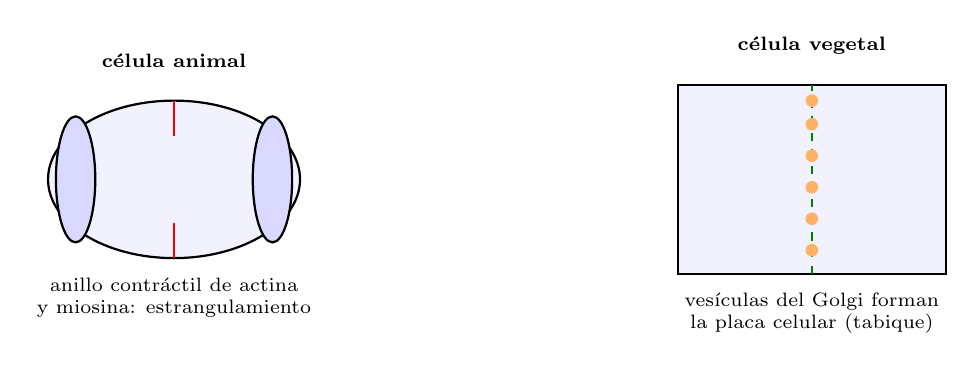
\begin{tikzpicture}
\tikzset{every node/.append style={align=center}}

\draw[thick, fill=blue!5] (1.6,1.8) ellipse (1.6 and 1.0); \draw[thick, fill=blue!15] (0.35,1.8) ellipse (0.25 and 0.8); \draw[thick, fill=blue!15] (2.85,1.8) ellipse (0.25 and 0.8);
\node[font=\bfseries\scriptsize] at (1.6,3.3) {célula animal}; \node[font=\scriptsize, align=center] at (1.6,0.3) {anillo contráctil de actina\\ y miosina: estrangulamiento};
\draw[thick, red] (1.6,2.8) -- (1.6,2.35); \draw[thick, red] (1.6,0.8) -- (1.6,1.25);
\draw[thick, fill=blue!5] (8.0,1.8) rectangle (11.4,3.0); \draw[thick, fill=blue!5] (8.0,0.6) rectangle (11.4,1.8);
\draw[thick, fill=blue!5] (8.0,0.6) rectangle (11.4,3.0);
\draw[thick, green!50!black, dashed] (9.7,0.6) -- (9.7,3.0);
\foreach \y in {0.9,1.3,1.7,2.1,2.5,2.8} {\fill[orange!60] (9.7,\y) circle (0.08);}
\node[font=\bfseries\scriptsize] at (9.7,3.5) {célula vegetal}; \node[font=\scriptsize, align=center] at (9.7,0.1) {vesículas del Golgi forman\\ la placa celular (tabique)};

\end{tikzpicture}
\end{document}
